\documentclass[10pt,a4paper]{article}
\usepackage[latin1]{inputenc}
\usepackage{amsmath}
\usepackage{amsfonts}
\usepackage{amssymb}
\usepackage{graphicx}
\usepackage[left=2.50cm, right=2.50cm, top=1.50cm]{geometry}

\usepackage[authoryear]{natbib}

\author{Fabian Schubert}
\title{Notes on Homeostatic Adaptation and Error Driven Adaptation in ESNs}
\begin{document}
	\maketitle
	
	\section{Introduction}
	Strategies for the optimization of ESN hyperparameters can be divided in two categories: supervised and unsupervised methods, where the first one utilizes an error signal, while the latter only uses information contained within the network dynamics.
	
	In the first part of our research, we investigated the possibility of defining an unsupervised homeostatic mechanism that controls the mean and variance of neuronal firing in such a way that the network acts in a regime that yields good performance in sequence learning tasks. This mechanism acts on two sets of parameters, biases $b_i$ and neural gain factors $a_i$. It should be emphasized that we did not attempt to define an arbitrarily complex measure that would be most suitable for optimization, e.g. from a machine learning perspective. Rather, we restricted ourselves to adhere to �biologically plausible' mechanisms. While no exact definition of this term exists, it embraced two aspects in our work:
	\begin{itemize}
		\item The dynamics of all variables must be local, i.e., they are bound to a specific neuron and may only access other variables that are locally accessible. In a strict sense, this consists of all other dynamic variables of the neuron itself and information about the activity of adjacent neurons. Being less restrictive, one could claim that it should also be possible to access aggregate or �mean-field' quantities, that average a property over the entire population.
		\item We use a time-discrete model where the state of a variable in the next step may only be determined by states of the previous step. This means that information about past states must be integrated dynamically.
	\end{itemize} 
	
	 Our approach was based on the assumption that network performance is optimal when the spectral radius of the effective recurrent connectivity, given by $a_i W_{ij}$, is close to, but slightly below $1$. We attempted to transfer this non-local measure into a condition that could be implemented in a biologically plausible way. 
	
	\section{Model}
	\subsection{Network dynamics}
	\begin{align}
		y_i(t) &= \tanh\left(a_i x_i(t) - b_i\right) \\
		x_i(t) &= \sum_{j=1}^N W_{ij} y_j(t-1) + \sum_{j=1}^{D_{\rm in}} W^{\rm u}_{ij} u_j(t) \\
		o_i(t) &= o^0_i + \sum_{j=1}^{D_{\rm out}} W^{\rm o}_{ij} y_j(t)
	\end{align}
	where $\mathbf{y}, \mathbf{x}, \mathbf{a}, \mathbf{b}  \in \mathbb{R}^N$, $W \in \mathbb{R}^{N \times N}$, $\mathbf{u} \in \mathbb{R}^{D_{\rm in}}$, $W^{\rm u} \in \mathbb{R}^{N \times D_{\rm in}}$, $\mathbf{o}, \mathbf{o}^0 \in \mathbb{R}^{D_{\rm out}}$ and  $W^{\rm o} \in \mathbb{R}^{D_{\rm out} \times N}$.
	
	Furthermore
	\begin{align}
		\mathrm{p}\left(W_{ij} = x\right) &= \begin{cases}
		\delta(x) & i=j \\
		p_{\rm r} \mathcal{N}\left(x,\mu=0,\sigma=\sigma_{\rm w}/\sqrt{Np_{\rm r}} \right) + (1-p_{\rm r}) \delta(x) & \mathrm{else}
		\end{cases} \\
		\mathrm{p}\left(W^{\rm u}_{ij} = x\right) &= \mathcal{N}\left(x,\mu=0,\sigma=1\right) \; .
	\end{align}
	
	Initially, we chose $N=1000$ as the network size, however, due to computational complexity, the results presented here are generated with a network of size $N=500$, unless stated otherwise. See Table~\ref{tab:net_params} for the standard network parameters.
	\begin{table}[h!]
		\centering
		\renewcommand{\arraystretch}{1.2}
		\caption{Standard network parameters.}
		\begin{tabular}{c|c|c|c|c}
			$N$ & $D_{\rm in}$ & $D_{\rm out}$ & $p_{\rm r}$ & $\sigma_{\rm w}$ \\ \hline
			500 & 1 & 1 & 0.1 & 1
		\end{tabular}
		\label{tab:net_params}
	\end{table}
	\subsection{Homeostatic Adaptation}
	For our homeostatic update mechanism, we use the following dynamics:
	\begin{align}
		b_i(t) &= b_i(t-1) + \epsilon_{\rm b} \left[y_i(t) - \mu^{\rm t}_i \right] \\
		\mu^{\rm y}_i(t) &= \left[1 - \epsilon_{\mu}\right] \mu^{\rm y}_i(t-1) + \epsilon_{\mu} y_i(t) \\
		a_i(t) &= a_i(t-1) + \epsilon_{\rm a} [{\sigma^{\rm t}_i}^2 - \left( y_i(t) - \mu^{\rm y}_i(t) \right)^2] \; .
	\end{align}
	See Table~\ref{tab:hom_params} for the standard values.
	
	\begin{table}[h!]
		\centering
		\renewcommand{\arraystretch}{1.2}
		\caption{Standard homeostasis parameters.}
		\begin{tabular}{c|c|c|c|c}
			$\epsilon_{\rm b}$ & $\epsilon_{\mu}$ & $\epsilon_{\rm a}$ & $\mu^{\rm t}_i$ & $\sigma^{\rm t}_i$\\ \hline
			$10^{-3}$ & $10^{-4}$ & $10^{-3}$ & $0.05$ & variable 
		\end{tabular}
		\label{tab:hom_params}
	\end{table}
	
	\section{Theory}
	We stated in the model description that all recurrent weights were drawn independently from a sparse Gaussian distribution. In some sense, of course, this is an assumption that already fulfills one of the conditions that is known to make ESNs work, namely a balance between excitation and inhibition. However, since adjusting gains does not provide a means to dynamically achieve this property, we had to take it as given.
	
	Furthermore, we assumed that all entries of the weight matrix were independently drawn from the same distribution. Under this assumption, using the circular law, it follows that setting all gain values to $1/\sigma_{\rm w}$ will result in a uniform unit circle distribution of eigenvalues. The situation is less clear if we allow the rows or columns of the matrix to follow different distributions, in particular---since we assumed to have zero mean---different variances. Numerically, we found that if
	\begin{equation}
		R_{\rm a} \equiv  \sum_i a^2_i \sigma^2_{{\rm w},i} = 1
	\end{equation}
	where $\sigma^2_{{\rm w},i}$ are the variances of individual rows of the matrix, the spectral radius will be unity. This observation was also reported and proven in \citep{Rajan2006}.
	
	From this observation, two question emerge: first, can we find local gain dynamics that can tune the global measure $R_{\rm a}$? And second, given the assumption that this constraint is fulfilled, does the particular distribution of gains affect the network performance?
	
	Since $R_{\rm a}$ is already a population average itself, we could simply argue that a biologically plausible mechanism that adjusts gains proportionally would be
	\begin{equation}
		a_i(t+1) = a_i(t) + \epsilon_{\rm a} a_i(t) \left[R^t_{\rm a} - R_{\rm a}(t) \right]
	\end{equation}
	where $R^t_{\rm a}$ is the spectral radius we would like to achieve.
	
	The question at hand is: could a diffusive neuromodulator encode the squared product of the neural gain and the variance of its synaptic weights? Or, alternatively, could this quantity be encoded in a different physical variable?
	
	\subsection{Spectral Radius Encoded in Input and Neural Activity}
	
	One possible way to encode the aforementioned quantity in physical way is based on the very general statement that each configuration of gains, weights and input statistics will yield a particular set of statistics for the resulting neural activity. Therefore, we hypothesized that it should be possible to establish an (approximate) description of the causal relation of these properties. In particular, this would potentially allow us to link a given value of $R_{\rm a}$, expressed as a function of gains and weights, to a corresponding set of input and neural activity statistics.
	
	Based on this approach, we came up with an approximate self-consistency equation that was based on the following assumptions/simplifications:
	
	\begin{itemize}
		\item We reduced the set of gains $a_i$ to single variable $a$.
		\item Every neuron receives statistically independent external input, which is however drawn from the same statistic characterized by the standard deviation $\sigma_{\rm ext}$. We assumed the mean input to be zero.
		\item Each neurons has the same homeostatic target variance.
		\item We ignore cross-correlations of activity in the neural population. Furthermore, we also assumed that each neuron has zero autocorrelation for $\tau \neq 0$.
		\item We ignore the small offset $\mu^{\rm t}_i$ in the mean activity.
	\end{itemize}
	 
	Under this assumptions, the networks fulfills a self-consistency equation given by
	
	\begin{equation}
	\sigma_{\rm t}^2=\int_{-\infty}^{\infty}
	{\rm dx}\tanh^2(ax) N_{\mu,\sigma}(x),
	\qquad\quad
	\sigma^2=\sigma_{\rm w}^2\sigma_{\rm t}^2+\sigma_{\rm ext}^2\,,
	\label{self_consistency_x}
	\end{equation}
	%
	where the distribution $N_{\mu,\sigma}(x)$ is 
	of the membrane potential $x$ is a Gaussian, with mean $\mu=0$
	and variance $\sigma^2$.
	A variable transformation $ax=z$ leads to
	%
	\begin{equation}
	\sigma_{\rm t}^2=\int_{-\infty}^{\infty}
	{\rm dz}\tanh^2(z) \frac{1}{\sqrt{2\pi\sigma_{\rm a}^2}}
	\mathrm{e}^{-z^2/2\sigma_{\rm a}^2}
	\qquad\quad
	\sigma_{\rm a}^2=a^2\big(\sigma_{\rm w}^2\sigma_{\rm t}^2+\sigma_{\rm ext}^2\big)\,,
	\label{self_consistency_z}
	\end{equation}
	%
	where the renormalized variance $\sigma_{\rm a}^2$ can
	be written as
	%
	\begin{equation}
	\sigma_{\rm a}^2=
	a^2\sigma_{\rm w}^2\big(\sigma_{\rm t}^2+\sigma_{\rm ext}^2/\sigma_{\rm w}^2\big)\,.
	\label{sigma_a_renormalized}
	\end{equation}
	%
	The gain $a$ is adapted such that (\ref{self_consistency_z})
	is fulfilled, defining a 2d-manifold in the $(\sigma_{\rm t},\sigma_{\rm ext},a)$ space. The relation (\ref{sigma_a_renormalized}) shows furthermore
	that the solution of (\ref{self_consistency_z}) depends on the ratio $\sigma_{\rm ext}/\sigma_{\rm w}$, which measures the relevance of the external driving with respect the recurrent synaptic connections. For convenience, we thus introduce $\sigma^\prime_{\rm ext} \equiv \sigma_{\rm ext}/\sigma_{\rm w}$.
	
	As a `sanity check', we ran a network simulation where the second and fourth approximation was actually exact. That is, we used Gaussian white noise with zero mean and $\sigma_{\rm ext}$	standard deviation for all neurons. Furthermore, the target mean was set to zero. Running the network for different pairs of external input variance and target variance, we got the results shown in Fig.~\ref{fig:gains_self_consist}.  
	
	%\begin{figure}
	%	\centering
	%	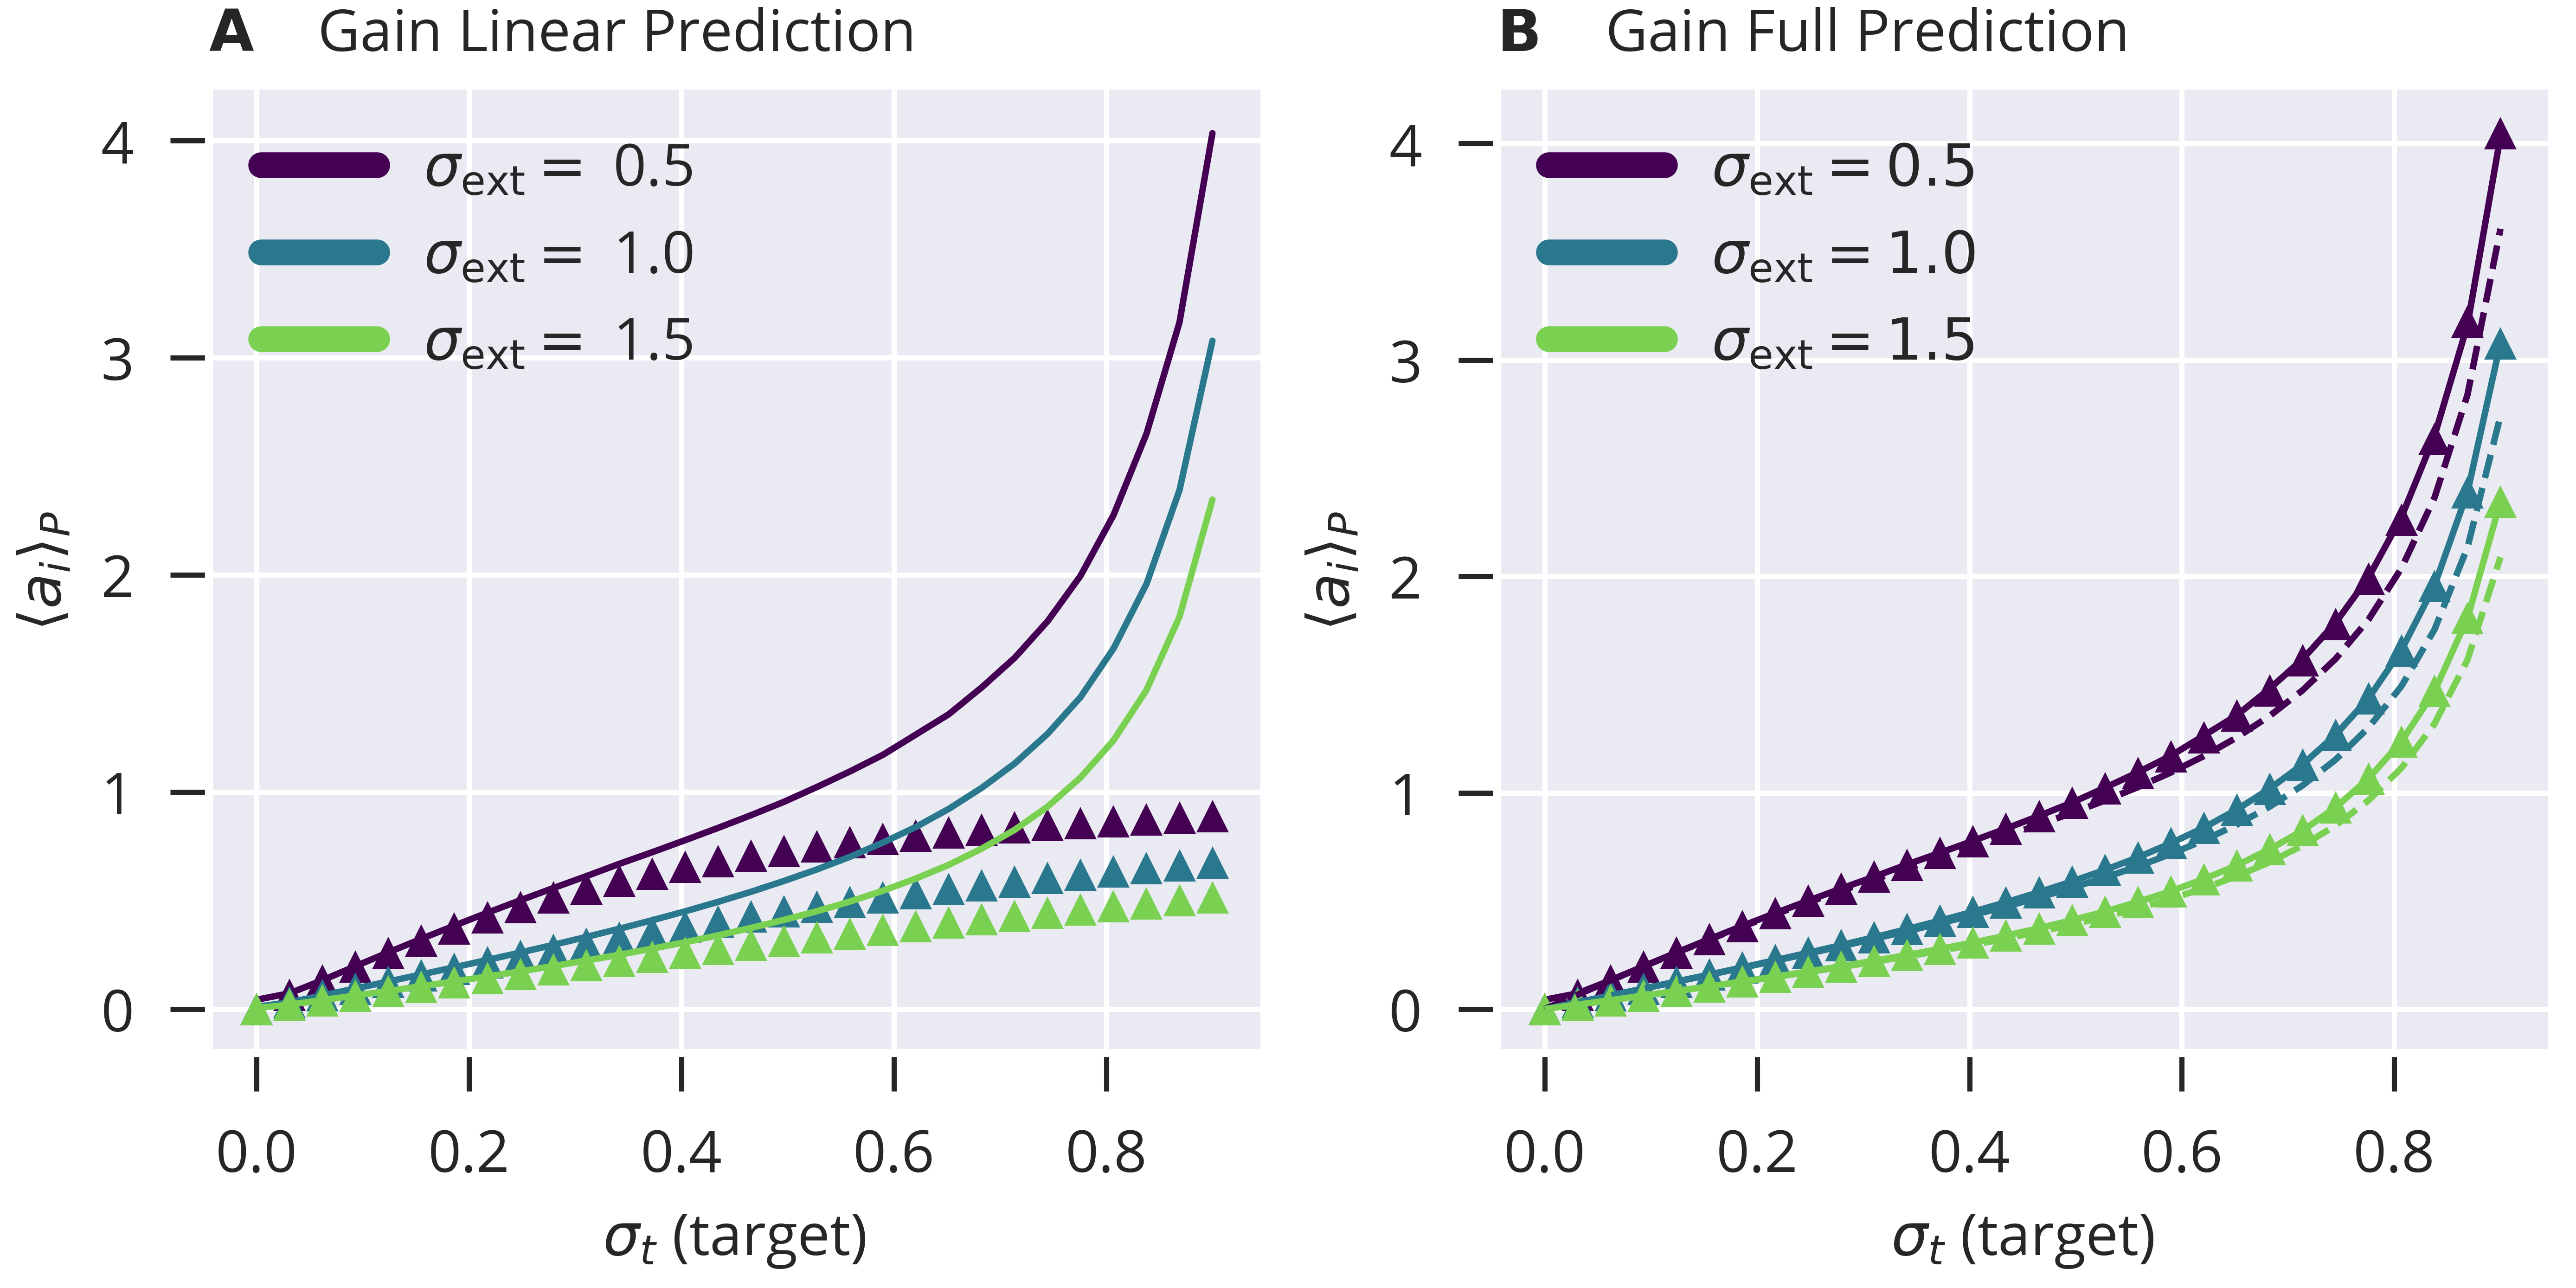
\includegraphics{../plots/std_in_std_target_sweep_fig_cut.png}
	%	\caption{Simulation for Gaussian Input. Triangles are numerical simulation, lines are the full mean field solutions, dashed lines are approximate solutions.}
	%	\label{fig:gains_self_consist}
	%\end{figure}
	
	\the\textwidth
		
	
			
	%%%%%%%%%%%%%%%%%%%%%%%%%%%%%%%%%%%%%%%%%%%%%%%%%%%%%%%
	\bibliographystyle{humannat}
	\bibliography{schubert_echo}
	%%%%%%%%%%%%%%%%%%%%%%%%%%%%%%%%%%%%%%%%%%%%%%%%%%%%%%%
	
\end{document}